% Pacotes que  fazem o sistema pegar, eh como o import do python
\documentclass[a4paper, 12pt]{article}
\usepackage[brazilian]{babel}
\usepackage[utf8]{inputenc}
\usepackage{amsmath}
\usepackage{cite}
\usepackage{indentfirst}
\usepackage{graphicx}
\usepackage[colorinlistoftodos]{todonotes}
\usepackage{hyperref}
\usepackage{gensymb}
\usepackage{tikz}
\usepackage{url}
\usepackage{enumerate}
\usepackage{float}
\usepackage{ragged2e}
\usetikzlibrary{babel}
\usetikzlibrary{calc,patterns,angles,quotes}

%Usage: \btable{table specs}{caption}{reference label}



\begin{document} %Comeco do documento

\begin{titlepage} 

\begin{figure}[H]
\centering

\includegraphics[width=1.75cm]{IFSC_USP.png} % Nome da Imagem 

\end{figure}
    \begin{center}
        Universidade de São Paulo \\
        
        Instituto de Física de São Carlos \\


\vspace{10pt}

        
        \vspace{85pt}
        
        
         \large\textbf{{Prática n: nome da Pratica }} % Titulo da Pratica 
        \vspace{160pt}
        
    \end{center}
    
    \begin{flushright}
        
         Nome Completo e Numero USP\\ % Colocar os nomes dos alunos aqui
         Nome Completo e Numero USP  \\
            Nome Completo e Numero USP
    \end{flushright}
    
    \begin{center}
        \vspace{\fill}
        23 de Outubro de 2017 % Onde eu coloco a data
    \end{center}
\end{titlepage}

\newpage
%\tableofcontents    % Posso ativar para ter a tabela de conteudo

\thispagestyle{empty}

\newpage
\pagenumbering{arabic}

%% Notas sobre a correção dos relatórios:
% i) Explicitar o número de medidas efetuadas; ii) Explicitar a precisão dos instrumentos na seção
% dos materiais empregados; iii) Discutir, nos resultados, qual dos métodos gerou o melhor
% resultado, o mais preciso, e indicar possíveis fontes de diferença entre os métodos empregados 
% que tenham levado às diferenças de precisão observadas;

\justifying

\section{Resumo}  % Colocar aqui o resumo do Trabalho 
\section{Introdução}
    

\begin{equation}
\label{eq:corda}
v = \sqrt{\frac{F}{\mu }}
\end{equation}
    
%Como colocar figuras
\begin{figure}[H]
\centering
\caption{}{Ondas estacionárias de deslocamento em uma corda presa em
ambos os extremos.}
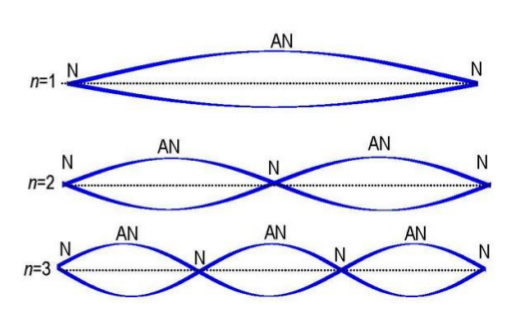
\includegraphics[width=10.0cm]{ondas_estacionarias.png}
\label{fig:ondas_estacionarias}  
\cite{lab}
\end{figure}

\section{Materiais e Métodos}.
\section{Resultados e discussão}

\vspace{0.75cm} % So para deixar um espaco maior entre os dados e o texto

%So para deixar mais afastado da equacao

\vspace{0.75cm} % So para deixar mais longe da tabelaa

\begin{table}[H] %Como fazer uma tabela
\caption{ Tabela relacionando os harmônicos com seus $f$ e suas $\lambda$}
\begin{center}
\scalebox{0.9}{
\begin{tabular}{c|c|c|c|c|c|c|c|c|c} \label{tab:primeira}
$n$  & 1 & 2 & 3 & 4 & 5 & 6 & 7 & 8 & 9 \\ 
$f$ $\pm 0.001$ Hz & 17.691 & 35.382 & 52.501 & 70.023 & 87.233 & 105.81 & 122.83 & 140.05 & 157.90 \\ 
$\lambda \pm 0.01$ & 1.32 & 0.66 & 0.45 & 0.33 & 0.27 & 0.22 & 0.19 & 0.17 & 0.15 \\ 
\end{tabular} 
}
\end{center}
\end{table}

\section{Conclusão}


\section{Bibliografia}
\begin{thebibliography}{9}
 
\bibitem{lab}
Laboratório de Física II - Livro de Práticas;

\bibitem{tipler}
Tipler, P. A., Mosca, G.. \textit{Física para Cientistas e Engenheiros.} Vol.1. LTC

\bibitem{moyses}
Nussenzveig, H. M.. \textit{Curso de Física Básica. } Vol. 2. Editora Blucher 

\end{thebibliography} 
\end{document}